\documentclass{standalone}
\usepackage[T1]{fontenc}
\usepackage[utf8]{inputenc}
\usepackage{pgf,tikz}
\usepackage{pgfplots}
\pgfplotsset{compat=1.9}

\begin{document}

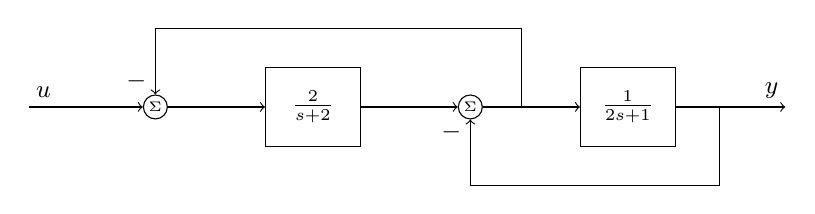
\begin{tikzpicture}[block/.style={rectangle, draw, minimum width=12mm, minimum height=10mm},
  sumnode/.style={circle, draw, inner sep=1pt},
  node distance=20mm]
  \small 
  \node[coordinate] (input) {};
  \node[sumnode, right of=input, node distance=16mm,] (sum) {\tiny $\Sigma$};
  \node[block, right of=sum] (G) {$\frac{2}{s+2}$};
  \node[sumnode, right of=G] (sum2) {\tiny $\Sigma$};
  \node[block, right of=sum2, ] (H) {$\frac{1}{2s+1}$};
  \node[coordinate, right of=H] (output) {};
 
  \draw[->] (input) -- node[ very near start, above] {$u$} (sum);
  \draw[->] (sum) -- node[] {} (G);
  \draw[->] (G) -- node[coordinate, pos=0.4] {} (sum2);
  \draw[->] (sum2) -- node[coordinate, pos=0.4] (fb) {} (H);
  \draw[->] (H) -- node[coordinate, pos=0.4] (fb2) {} node [above, very near end] {$y$} (output);

  \draw[->] (fb) -- ++(0, 10mm) -| node[left, pos=0.9] {$-$} (sum); 
  \draw[->] (fb2) -- ++(0, -10mm) -| node[left, pos=0.9] {$-$} (sum2); 


  
\end{tikzpicture}
\end{document}
